\chapter{Interactive Musical Score}

\section{Introduction}

\subsection*{Overview}

In this work, we introduce the Interactive Score, a novel instrumental device for children's solfege
learning. Paper scores are overlaid onto a staff drawn with conductive ink and
connected to an Adafruit musical box. Pressing a note in the score triggers its sound,
and running fingers over the notes plays a melody.


\subsection*{Motivation}

Learning to read music from the score is an essential part of Western classical music
training. Traditionally, children learn the different music notes by singing or playing
notes on an instrument, guided by a teacher. We envision a way for children to learn
the correspondence between notation and sound by directly touching the score.
The Interactive Score is effortless to use and allows children to make discoveries on
their own. The correspondence between the visual, the tactile, and the sound can aid
in learning.

\section{Related work}

\subsection{Musical Mental Projection}

Musical imagery, or the ability to create an image of sound in our minds, is an essential
skill for all musicians. For example, brass, winds, strings, and singers imagine the
pitch of an upcoming note to make it easier to play it and determine the distance from
the previous note
\cite{zatorre2005mental}. Composers and arrangers also use musical imagery when creating
a new piece. Musical imagery training has been shown to improve the ability to follow
the upward and downward movements of the tonal contour of a musical phrase or
imagined tune
\cite{weber1986musical}.

Ear training" (or solfège) has traditionally been part of the curriculum of most music
schools. An important part of solfège is the ability to read music notation and imagine
how it is supposed to sound. We are interested in teaching this skill to children.

\subsection{Traditional approaches}

\subsection{Tangible Interactive Medias}

\section{General Architecture}

\subsection{Overview}

Online many digital music learning applications, which run on screen-based devices,
our design augments a traditional paper score. Children already spend a considerable
time in front of screens, which can harm their eyes from a young age. Paper is flexible,
lightweight and easily transportable, and the incorporation of electronic circuits in
paper has shown its attractiveness to children
\cite{hershman2018light}.

\begin{figure}[h]
    \centering
    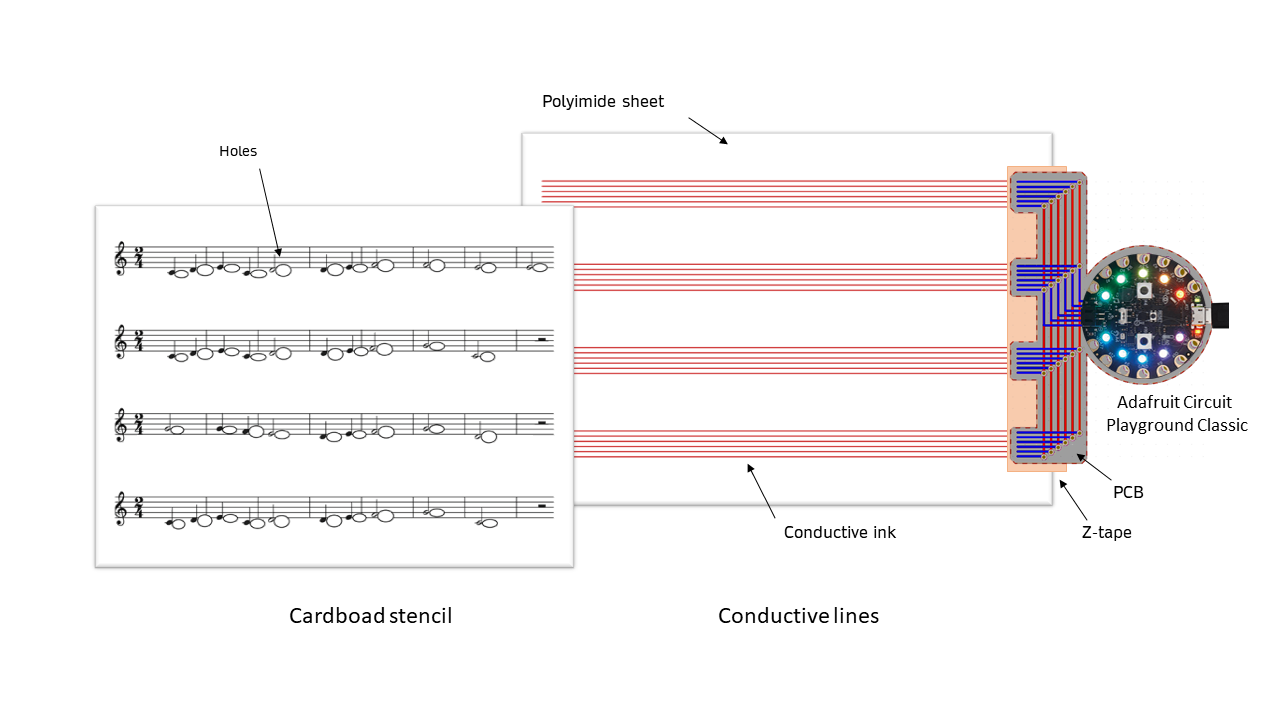
\includegraphics{images/IS_schema.png}
    \caption{Interactive Musical Score architecture.}
    \label{fig:IS_schema}
\end{figure}

The demonstrator supplies the electronic part (substrate and PCB) during the
showcase. He places a partition (a cardboard stencil) on top of the substrate (where
the conductive lines are located). He plays the music and then changes it to another
one

\subsection{System Design}

The Interactive score consists of two thin layers. The first layer is the traditional sheet
music, printed on cardstock paper, with holes punched for each note. Under this sheet
is a polyimide substrate with conductive lines printed on it. The ink paths are 1mm
thick, 5cm in length, with a resistance of 0.07 Ohms. The conductive lines are printed
using a simple inkjet printer equipped to print with conductive ink and are sintered at
180°C for 73 minutes. This process allows the quick production of flexible circuits \cite{khan2019soft}.
The conductive lines are connected to an Adafruit Circuit Playground printed circuit
board (PCB) using double-sided “z-tape.”
When the user touches a note on the top layer, contact is made between the finger and
the conductive lines through the holes in the cardstock. The signal travels through the
ink paths and the z-tape to the PCB, which detects a potential difference using
capacitive touch and plays the relevant note. The detection of several simultaneous
signals on multiple pins allows the playing of eleven different notes with only six lines.

\subsection{Electronic Music Box}

\subsection{Conductive Sheet Manufacturing}

\subsection{Integration and Usability}

\subsubsection{Ability to change the score}

Its ease of interchangeability characterizes the paper score. It is easy to produce. It
can easily be removed from the box and another one placed in its place to play a
different melody. All the electronic parts (substrate, PCB, microcontroller) are
independent of the paper score. The user can change it without changing the code or
the rest of the device. The sheet music has the exact dimensions of the substrate.
Therefore, it is simple to place the two precisely on top of each other to align the
holes with the ink lines.
\subsubsection{Ability to improvise} 

The user has the capacity to improvise by not playing the notes in the same order.
The project allows a great deal of modularity in its use. Just by touching specific
notes at certain times, users can experiment with different rhythms and melodies
and reconstruct a piece from a few notes.
With a simple score including an ascending scale, he can try his hand at composition.
As the microcontroller code is configured to play melodies in C major, it is not
possible to create dissonance.


\section{Applications and Evaluation}

\section{Discussion}

\subsection{Attractivity}

\subsection{Musical Imagery learning}

\subsection{Mobilising multiple intelligences}

\section{Conclusion}

\subsection{Limitations}

\subsection{Future works}

A "musical tutorial" mode will soon be added so that the user can listen to the score's
music before having to play it. This will allow the user to assimilate the musical rhythm
(the time between playing each note) with the physical rhythm (the time between
pressing notes).
The electronic PCB/microcontroller part will be redesigned to no longer integrate an
Adafruit Circuit Playground but a much smaller circuit entirely made by us. The
learner can replace each component in case of a problem. It will be possible to
improve the speaker's quality and connect the device to Bluetooth or Wi-Fi to play
music at a distance.
We are currently looking for partnerships in children's education to research
experimentations on the impact of this interactive score on music assimilation. Several
parameters would be evaluated, such as the concentration level, playing time, and
knowledge retention. We will consider different strategies to transcript musical-rhythmic on this interactive score.